\documentclass{minimal}
%  1360x768
\usepackage[paperheight=3.84in,paperwidth=6.8in,left=0.in,top=0.in,bottom=0in]{geometry}
\usepackage{tikz}
\usepackage{xcolor}
\usepackage{graphicx}
\usepackage[T1]{fontenc}
\usepackage{tgbonum}
\fontfamily{qcr}


% \renewcommand\normalsize{\fontsize{12pt}{14pt}\selectfont}   
\newcommand{\titlefont}{\fontsize{17.28pt}{40pt}\selectfont}   
% \newcommand{\titlefont}{\fontsize{14pt}{14pt}\selectfont} 
\newcommand{\subtitlefont}{\fontsize{12pt}{24pt}\selectfont} 
\setlength{\parindent}{0in}  
% \pagenumbering{arabic}  % but no page numbers are printed because:
% \pagestyle{empty}   

\begin{document}

\begin{tikzpicture}
    % \node[anchor=west] at (-0.1,0.1) {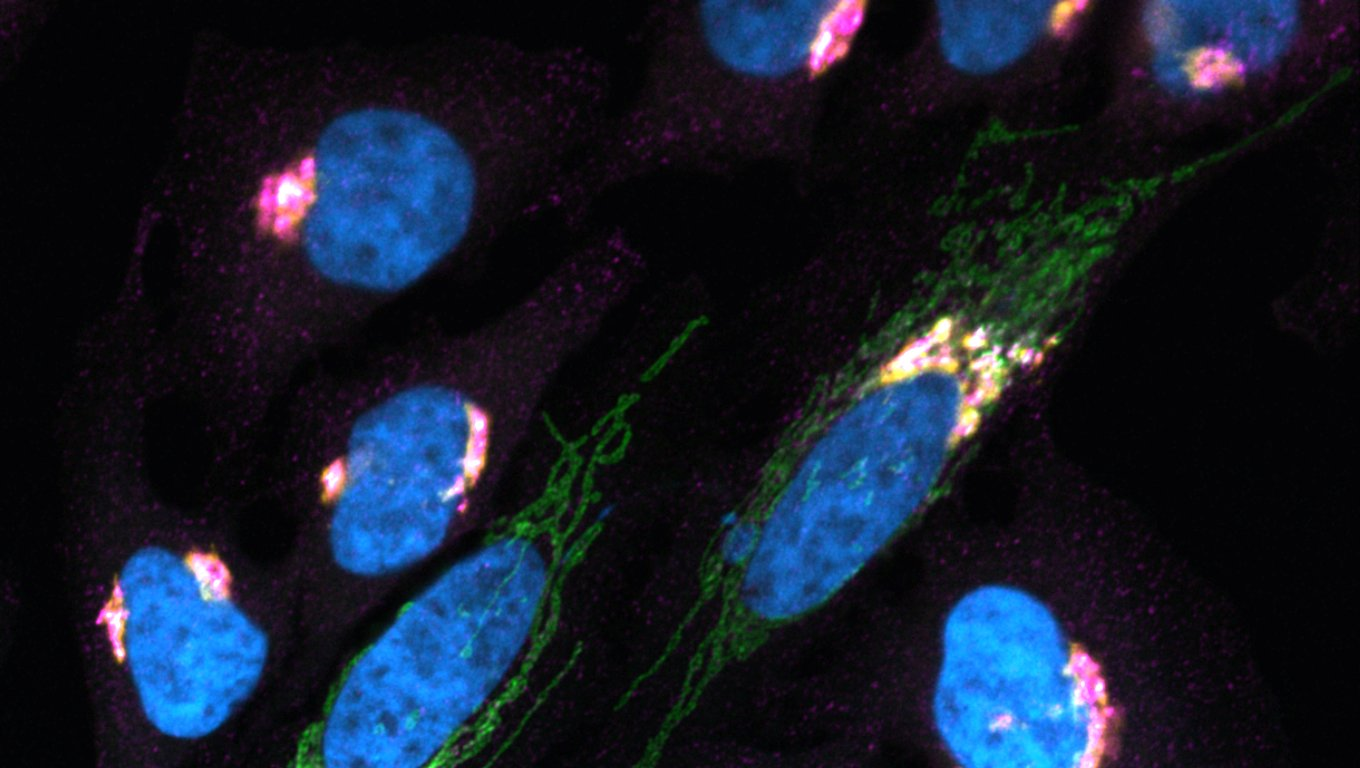
\includegraphics[width=6.8in]{artwork/background.jpg}};
    \node[anchor=west] at (0in,-0.0in) {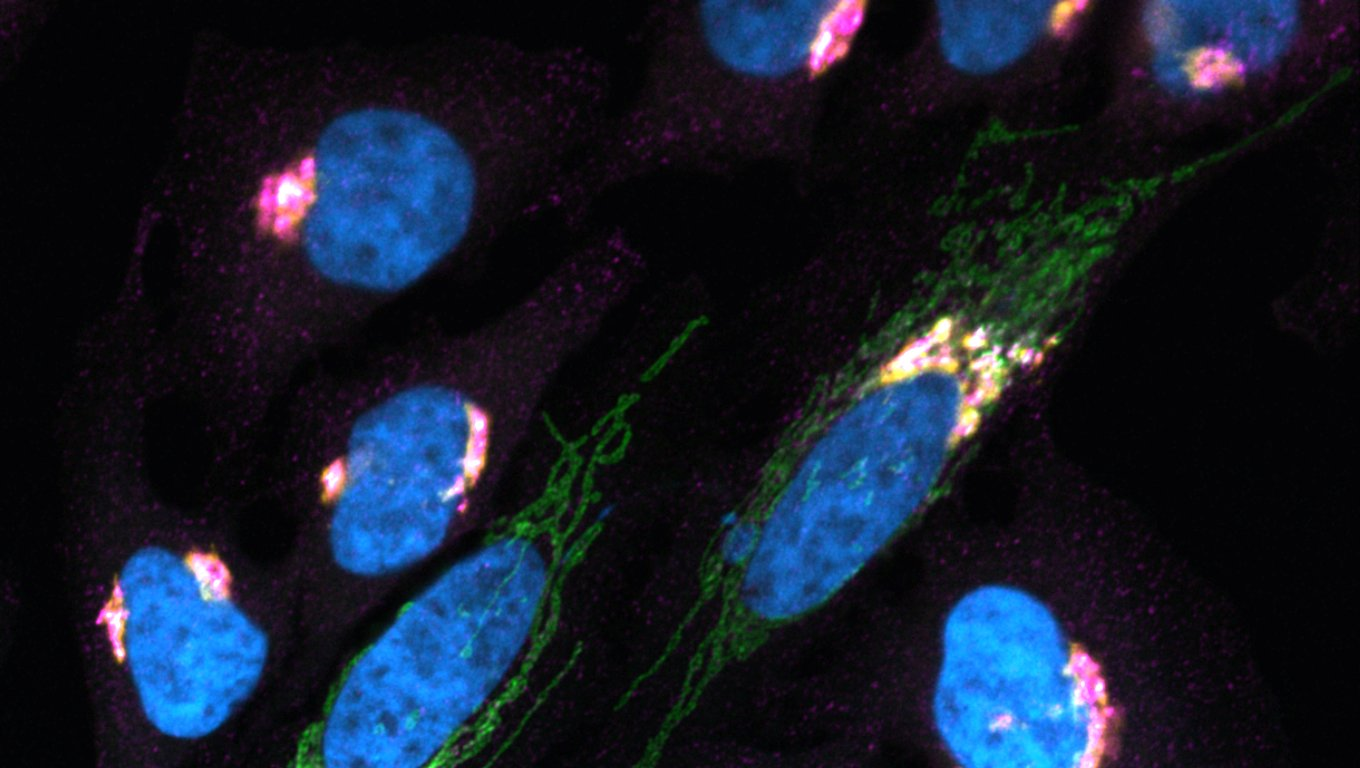
\includegraphics[height=2.1in,angle=90]{artwork/background.jpg}};
    % \fill[yellow!30] (6.4in,-1.2in) rectangle (6.8in,-1.4in);
    % \node[anchor=west] at (3.2in,-0.0in) {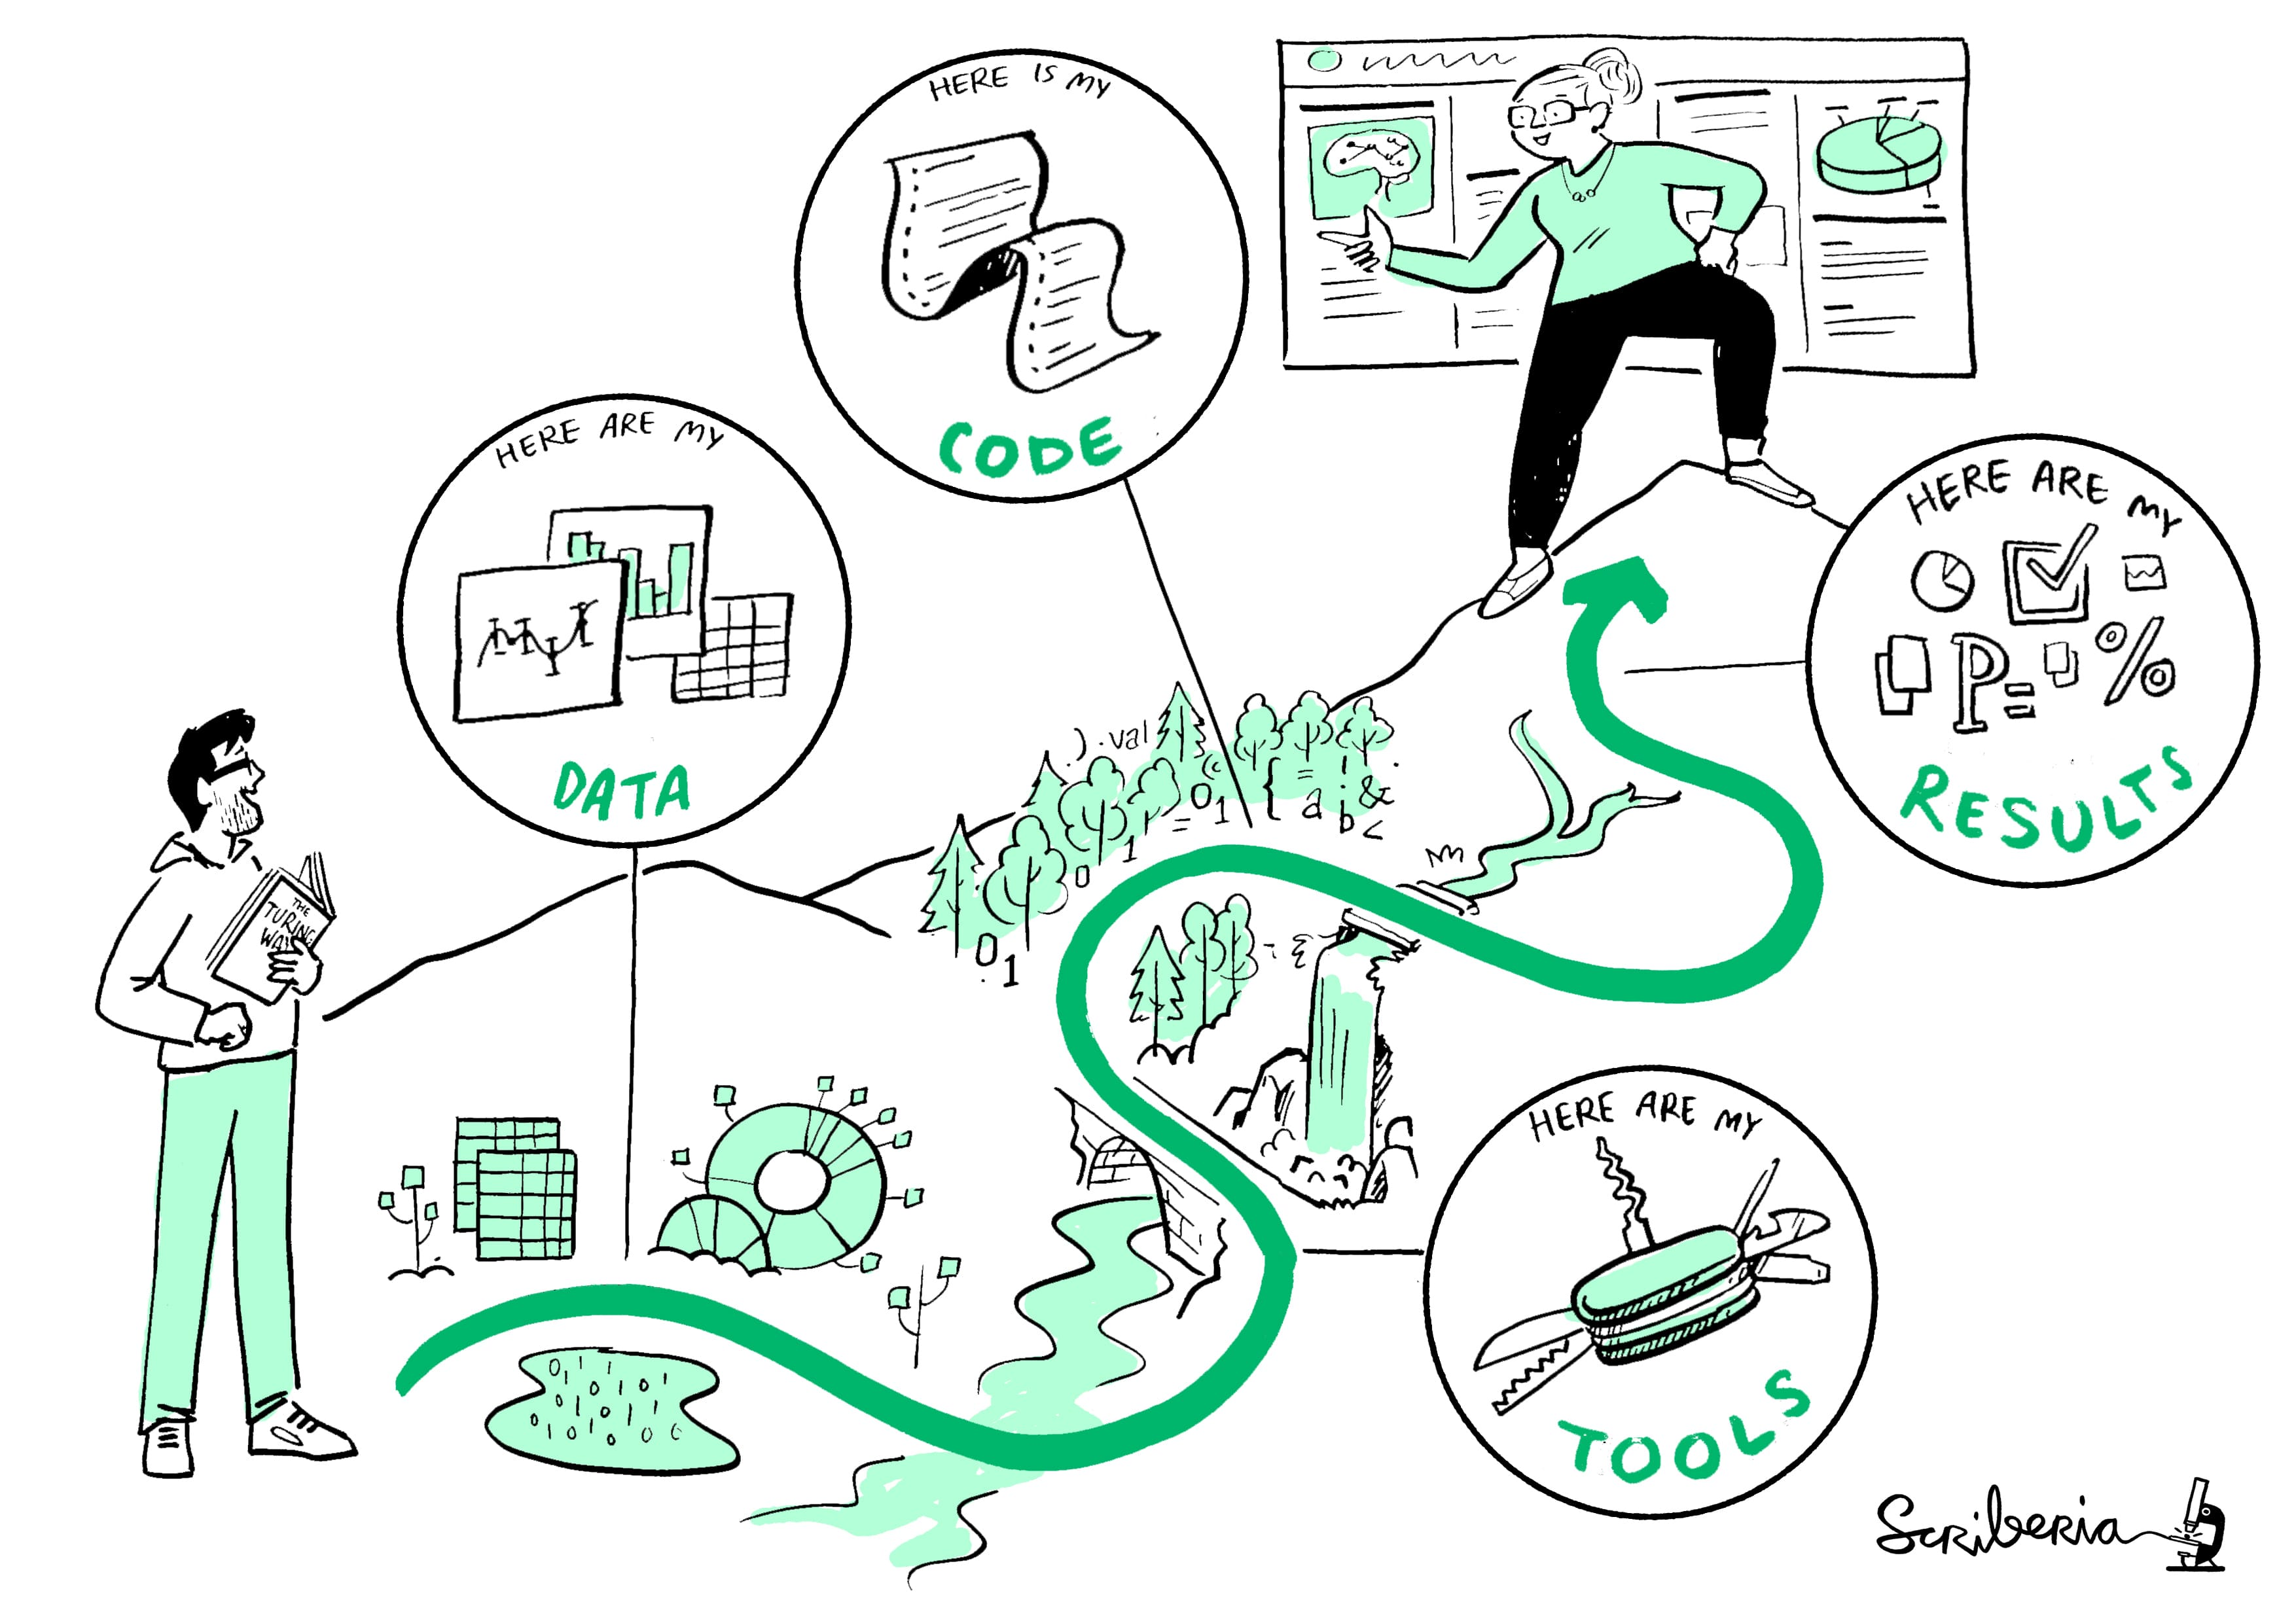
\includegraphics[width=3in]{artwork/reproducibility.jpg}};
    % \node[anchor=west] at (0in,1.7in) {\textbf{\titlefont Hands-on Nikon NIS-Elements GA3 Training}};
    \node[anchor=west] at (2.3in,0.2in) {
        \begin{minipage}{4.in}
            \textbf{\titlefont Nikon Elements GA3 Training}

            \vspace{0.4cm}
            
            \textbf{\subtitlefont Build Your Own Workflows}
            \vspace{0.6cm}
        
            \textbf{June 2nd and 3rd}
            
            \vspace{0.6cm}
            \textbf{Topics:} 
            Preprocessing, Segmentation, AI segmentation, Tracking, Object parenting, Batch processing, \dots

            \vspace{1cm}

            \begin{center} 
                
\includegraphics[width=0.75in]{artwork/qr.png}
            \end{center}
        \end{minipage}
    };

\end{tikzpicture}







% \begin{tikzpicture}
%     \node[align=left] at (0,5){\LARGE \bf Hands-on Nikon NIS-Elements GA Training};
%     \node[align=left] at (-1,4){\Large Build Your Own Workflows};
%     \node[align=left] at (0,3){June 2nd and 3rd};
% \end{tikzpicture}

\end{document}